\documentclass[11pt, a4paper]{article}

% --- Packages ---
\usepackage[utf8]{inputenc} % Encoding
\usepackage{amsmath, amssymb, amsthm} % Advanced math typesetting
\usepackage{physics} % Useful commands for physics (derivatives, vectors, braket)
\usepackage{graphicx} % For including diagrams and images
\usepackage{geometry} % Page margins
\usepackage{siunitx} % For proper formatting of SI units
\usepackage{fancyhdr} % Custom headers and footers
\usepackage{xcolor} % For blocks of color
\usepackage{enumitem} % For enumerated lists with letters
\usepackage{float} % For figure strict positioning
\usepackage{parskip} % Remove the indentation and add space between paragraphs

% --- Page Setup ---
\geometry{top=2.5cm, bottom=2.5cm, left=2.5cm, right=2.5cm}
\pagestyle{fancy}
\fancyhf{} % Clear all default header and footer fields
\fancyhead[L]{\textbf{José Carlos López Henestrosa}}
\fancyhead[R]{Inteligencia artificial - PEC1}
\fancyfoot[C]{\thepage} % Page number at the bottom center

% --- Custom Environments ---
\newenvironment{problem}[1][Cuestión]{
	\vspace{0.5cm}
	\noindent{\Large\bfseries #1} \par\vspace{0.5cm}
}{
	\vspace{0.5cm}
}

\begin{document}
	% --- Title block ---
	\begin{center}
		\Large{ \textbf{PEC1} } \\
		\vspace{0.5cm}
		\normalsize{\textbf{Autor:} José Carlos López Henestrosa}
	\end{center}

	\vspace{1cm}
	\hrule
	\vspace{1cm}

	% --- Exercise 1 ---
	\begin{problem}[Cuestión 1 (20\%)]
		Si la heurística es admisible pero no consistente, al ejecutar el algoritmo A*, ¿pueden volver a aparecer en \textit{Abiertos} nodos que ya están en \textit{Cerrados}? 

		Proponed un grafo y un heurístico que ejemplifique la respuesta que se ha dado (\textit{no sirven los ejemplos de los materiales, quiero que os lo penséis vosotros; se pueden encontrar grafos pequeños que sirven de ejemplo}). Hacedlo muy detallado: argumentad por qué el heurístico es o no admisible, es o no consistente y realizad una ejecución manual del A* (enseñando a cada paso los \textit{Abiertos} y los \textit{Cerrados}).

		{ \color{blue} 
			Si una heurística es admisible pero no consistente, implica que el algoritmo A* puede encontrar un camino hacia un nodo que ya está en la lista de \textit{Cerrados} con un coste menor ($g$) al que tenía cuando se expandió originalmente. Por lo tanto, sí que pueden aparecer en nodos \textit{Abiertos} nodos que ya están en \textit{Cerrados}. 

			Para explicarlo usando un ejemplo práctico, nos apoyamos sobre el grafo $Z$, el cual contiene 4 nodos: $S$ (nodo inicial), $A$, $B$ y $G$ (nodo objetivo). Vamos a atribuirles los siguientes costes a sus aristas:

			\begin{itemize}
				\item Coste$(S,B) = 5$
				\item Coste$(S,A) = 2$
				\item Coste$(A,B) = 2$
				\item Coste$(B,G) = 20$
			\end{itemize}

			Con estos costes, el coste real óptimo para llegar al objetivo $G$ desde cada nodo (lo cual denotamos como $h^*$) es:

			\begin{itemize}
				\item $h^*(G) = 0$
				\item $h^*(B) = 20$ (camino $B \to G$) 
				\item $h^*(A) = 2 + 20 = 22$ (camino $A \to B \to G$)
				\item $h^*(S) = 2 + 2 + 20 = 24$ (camino óptimo $S \to A \to B \to G$)
			\end{itemize}

			A partir de estos costes, proponemos la siguiente función heurística ($h$) para cada nodo:

			\begin{itemize}
				\item $h(G) = 0$
				\item $h(B) = 5$
				\item $h(A) = 20$
				\item $h(S) = 24$
			\end{itemize}

			Sabemos que una función heurística es \textbf{admisible} si nunca sobrestima el coste real de alcanzar el objetivo desde un nodo. Si comparamos nuestro heurístico $h(n)$ con el coste real $h^*(n)$, obtenemos lo siguiente:

			\begin{itemize}
				\item $h(G) = 0 \le 0$
				\item $h(B) = 5 \le 20$
				\item $h(A) = 20 \le 22$
				\item $h(S) = 24 \le 24$
			\end{itemize}

			Como podemos apreciar, para todos los casos se cumple que $h(n) \le h^*(n)$. Por lo tanto, el heurístico es \textbf{admisible}. Al ser optimista, sabemos que el algoritmo A* completo siempre encontrará la solución más óptima.

			Por otro lado, sabemos que un heurístico es \textbf{consistente} si para todo par de nodos conectados (por ejemplo, de $x$ e $y$) el heurístico de $x$ es menor o igual al coste de ir de $x$ a $y$ más el heurístico de $y: h(x) \le \text{Coste}(x,y)+h(y)$. Dicho de otra forma, avanzar hacia un vecino no debe hacer decrecer la $h$ más de lo que crece el coste real $g$. Por ejemplo, si evaluamos la arista de $A$ a $B$:

			$$
			h(A) \le \text{Coste}(A,B) + h(B) \to 20 \le 2 + 5 \to 20 \le 7
			$$

			La desigualdad no se cumple, lo cual implica que el heurístico en el nodo $A$ decrece bruscamente al pasar al nodo $B$. Por ello, el heurístico es \textbf{inconsistente}.

			Por último, aplicamos el algoritmo A* completo, donde si un sucesor ya está en la lista de \textit{Cerrados} pero presenta un coste $g$ menor al que tenía cuando se cerró, se extrae de \textit{Cerrados} y se reabre en \textit{Abiertos} con su coste actualizado. Evaluaremos los nodos sumando $g + h = f$, donde $g$ es el coste desde el estado inicial nodo objetivo y $h$ es la estimación. Continuamos con la notación de mantener solo el nodo de menor coste si hay duplicados en \textit{Abiertos}.

			\textbf{Paso inicial:} Inicializamos con el nodo origen.
			\begin{itemize}
				\item \textbf{Abiertos(0):} $(S, 0 + 24) \to (S,24)$
				\item \textbf{Cerrados(0):} $\emptyset$
			\end{itemize}

			\textbf{Paso 1:} Extraemos $S$. Sus sucesores son $A$ ($g=2$) y $B$ ($g=5$).
			\begin{itemize}
				\item \textbf{Abiertos(1):} $(B, 5 +5),(A,2+10) \to (B,10),(A,24)$
				\item \textbf{Cerrados(1):} $(S,24)$
			\end{itemize}

			\textbf{Paso 2:} Extraemos $B$, ya que tiene el menor valor de $f$ ($10$). Su único sucesor es $G$ con coste $g = 5+20 =25$.
			\begin{itemize}
				\item \textbf{Abiertos(2):} $(A,22),(G,25+0) \to (A,22),(G,25)$
				\item \textbf{Cerrados(2):} $(S,24),(B,10)$
			\end{itemize}

			\textbf{Paso 3:} Extraemos $A$, ya que $f = 22 < 25$. Su sucesor es $B$ con un nuevo coste:

			$$g_{\text{nuevo}} = g(A) + \text{Coste}(A,B) = 2 + 2 = 4$$

			El nodo $B$ ya estaba en el conjunto de \textit{Cerrados}. Sin embargo, al comparar su coste anterior ($g=5$) con su nuevo coste descubierto a partir de $A$ ($g=4$), vemos que el nuevo camino es mejor ($4<5$). Por lo tanto, sacamos a $B$ de la lista de \textit{Cerrados} y lo devolvemos a \textit{Abiertos}. Ahora su función se convierte en $f(B) = 4+5=9$.

			\begin{itemize}
				\item \textbf{Abiertos(3):} $(B,4+5),(G,25) \to (B,9),(G,25)$
				\item \textbf{Cerrados(3):} $(S,24),(A,22)$ (ya no está $B$)
			\end{itemize}

			\textbf{Paso 4:} Extraemos $B$, ya que $f = 9$. Su sucesor es $G$ con un nuevo coste:

			$$g = g(B) + \text{Coste}(B,G) = 4+20 = 24$$

			El nodo $G$ ya estaba en el conjunto de \textit{Abiertos} con $f=25$. Al encontrar un camino mejor ($f=24$), nos quedamos con el de menor coste.

			\begin{itemize}
				\item \textbf{Abiertos(4):} $(G,24+0) \to (G,24)$
				\item \textbf{Cerrados(4):} $(S,24),(A,22),(B,9)$
			\end{itemize}

			\textbf{Paso 5:} Extraemos $G$. Al ser el estado objetivo, el algoritmo termina su ejecución correctamente. La solución hallada es $S \to A \to B \to G$ con coste óptimo de 24.

			Cabe destacar que si hubiésemos utilizado el algoritmo A* simplificado, habríamos ignorado los nodos \textit{Cerrados} sin revisar sus costes, por lo que el algoritmo jamás habría reabierto el nodo $B$. Esto implicaría que el algoritmo finalizase prematuramente devolviendo la ruta errónea y subóptima $S \to B \to G$ con coste 25.
		}

			\vspace{0.5cm}
		\end{problem}

	% --- Exercise 2 ---
	\begin{problem}[Cuestión 2 (10\%)]
		En el algoritmo A* (suponiendo que un heurístico $h2$ domina sobre un heurístico $h1$), ¿cómo afecta la dominancia de una heurística $h2$ sobre otra heurística $h1$ al número de nodos expandidos?

		{ \color{blue} 
			Analizamos la condición de expansión de nodos del algoritmo A*. Si suponemos que la solución óptima tiene un coste total $k$, A* deberá expandir todos los nodos cuya estimación de coste total $(g(n)+h(n))$ sea menor que $k$. Aplicando esto a ambas heurísticas, sabemos que si un nodo $n$ se expande usando la heurística $h2$, significa que $\text{coste}(\text{origen},n)+h2(n)<k$. Dado que $h1(n)$ es menor o igual a $h2(n)$ debido a la dominancia, por pura lógica matemática también se cumplirá que $\text{coste}(\text{origen},n)+h1(n)<k$. Por lo tanto, todo nodo que se expanda con la heurística $h2$ también será expandido por $h1$.

			Sin embargo, a la inversa no sucede lo mismo. Pueden existir nodos donde $\text{coste}(\text{origen},n)+h1(n)<k$, pero que al ser evaluados con la heurística más informada resulten en $\text{coste}(\text{origen},n)+h2(n) \ge k$. En estos casos, la heurística $h1$ provocaría la expansión innecesaria de esos nodos extra, mientras que la heurística dominante $h2$ los descartaría, haciendo la búsqueda mucho más rápida.

			Debido a esta clara ventaja en la eficiencia, los materiales señalan un truco útil: si disponemos de varias funciones heurísticas admisibles, se puede construir una nueva heurística que las domine a todas calculando el valor máximo de todas ellas para cada nodo evaluado. Es decir, $h(n)=\max(h1(n),h2(n),...)$.

			Como conclusión, en el algoritmo A*, si una función heurística $h2$ domina a otra heurística $h1$ (lo que significa que $h2(n) \ge h1(n)$ para todo nodo $n$), la búsqueda utilizando $h2$ siempre será \textbf{igual o más eficiente} porque provocará la expansión de un número menor o igual de nodos que $h1$.
		}

		\vspace{0.5cm}
	\end{problem}

	% --- Exercise 3 ---
	\begin{problem}[Cuestión 3 (10\%)]
		¿Qué pasa si cambiamos el algoritmo A* y consideramos un factor constante que multiplique el heurístico: $f(n) = g(n) + W \cdot h(n)$ con $W > 1$?

		{ \color{blue} 
			Al multiplicar la heurística por un factor $W > 1$, la nueva función heurística efectiva, $h'(n) = W \cdot h(n)$, sobreestima el coste real hacia el objetivo, lo cual va en contra de la propiedad de admisibilidad. En consecuencia, el algoritmo puede no encontrar el camino óptimo. No obstante, si la heurística original $h(n)$ era admisible, el coste de la solución encontrada, $C$, tendrá un límite superior respecto al coste óptimo $C^*$:$$C \le W \cdot C^*$$ 

			Por otra parte, al ponderar $h(n)$ con un valor mayor a 1, el algoritmo le da más importancia a la estimación del coste restante que al coste ya acumulado $g(n)$. Esto altera la estrategia de búsqueda y le atribuye un carácter más "voraz". En lugar de expandir frentes de búsqueda amplios para la optimalidad, como hace A* estándar, la búsqueda se dirige de forma mucho más directa hacia el nodo objetivo. Es por ello que el número total de nodos expandidos se reduce drásticamente, por lo que, en términos computacionales, el tiempo de ejecución y el consumo de memoria \textbf{mejoran}.
		}

		\vspace{0.5cm}
	\end{problem}

	% --- Exercise 4 ---
	\begin{problem}[Cuestión 4 (10\%)]
		¿Cuál sería el comportamiento del algoritmo A* si tuviéramos $h(n) = h^*(n)$ (el coste real exacto)?

		{ \color{blue} 
			Dada una heurística $h(n)=h^*(n)$ (es decir, la estimación del coste al objetivo es exactamente igual al coste real), el comportamiento del algoritmo A* sería óptimo, directo y eficiente. Es un indicador de que la función de evaluación $f(n)=g(n)+h(n)$ calcularía el coste total exacto del camino óptimo desde el nodo inicial hasta el objetivo pasando por el nodo $n$. Como resultado, A* nunca expandiría un nodo que no formara parte del camino óptimo final.

			Durante el desarrollo del algoritmo, este seguiría el camino óptimo como si estuviera guiado por un láser. En cada paso, el nodo con el menor valor de $f(n)$ en la lista de \textit{Abiertos} sería siempre el siguiente nodo correcto en la ruta hacia el objetivo.

			En términos de tiempo y memoria, el algoritmo se vuelve casi lineal con respecto a la longitud de la solución. Solo guardaría y expandiría lo necesario.

			El único escenario donde A* con una heurística perfecta exploraría más de un solo camino directo se da si existen múltiples caminos óptimos con exactamente el mismo coste total. En ese caso, todos los nodos de esos caminos empatados tendrían el mismo valor exacto de $f(n)$, y el algoritmo podría expandirlos simultáneamente dependiendo de cómo gestione los empates.
		}

		\vspace{3cm}
	\end{problem}

	% --- Exercise 5 ---
	\begin{problem}[Cuestión 5 (30\%)]
		Dado el grafo dirigido:

		\begin{figure}[H]
			\centering
			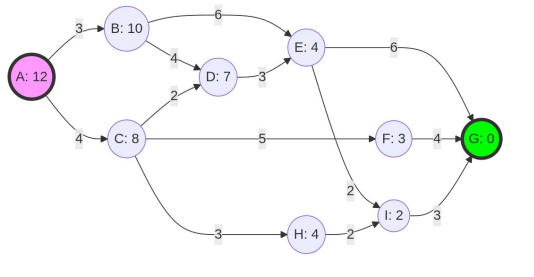
\includegraphics[width=13cm]{imagenes/cuestion-5.png}
		\end{figure}

		con el coste detallado en las aristas y la función heurística $h$ detallada en los nodos.

		Utilizad la \textbf{búsqueda ávida} y \textbf{búsqueda A*} para encontrar un camino desde el nodo \textit{A} hasta el nodo \textit{G}, y comparad las soluciones. \textit{Es necesario detallar las búsquedas en vuestra solución con las listas de nodos cerrados y abiertos (tenéis ejemplos en las soluciones de las PECs resueltas de otros semestres}.

		¿Es admisible esta heurística? Aplicad el algoritmo de Dijkstra (¡que deberíais conocer!) para justificarlo. ¿Es consistente?

		{ \color{blue} 
			\textbf{Aplicación de la búsqueda ávida}:

			\begin{itemize}[label={}]
				\item $[['A', 12]]$
				\item $[]$

				\vspace{0.20cm}

				\item $[['C', 8], ['B', 10]]$
				\item $[['A', 12]]$

				\vspace{0.20cm}

				\item $[['F', 3], ['H', 4], ['D', 7], ['B', 10]]$
				\item $[['C', 8], ['A', 12]]$

				\vspace{0.20cm}

				\item $[['G', 0], ['H', 4], ['D', 7], ['B', 10]]$
				\item $[['F', 3], ['C', 8], ['A', 12]]$

				\vspace{0.20cm}

				\item $[['H', 4], ['D', 7], ['B', 10]]$
				\item $[['G', 0], ['F', 3], ['C', 8], ['A', 12]]$
			\end{itemize}

			\textbf{Resultado:}

			\begin{itemize}[label={}]
				\item \textbf{Camino:} $A \rightarrow C \rightarrow F \rightarrow G$
				\item \textbf{Coste total:} $12$
			\end{itemize}

			\vspace{2cm}

			\textbf{Aplicación de la búsqueda A*}:

			\begin{itemize}[label={}]
				\item $[['A', 12]]$
				\item $[]$

				\vspace{0.20cm}

				\item $[['C', 12], ['B', 13]]$
				\item $[['A', 12]]$

				\vspace{0.20cm}

				\item $[['H', 11], ['F', 12], ['B', 13], ['D', 13]]$
				\item $[['A', 12], ['C', 12]]$

				\vspace{0.20cm}

				\item $[['I', 11], ['F', 12], ['B', 13], ['D', 13]]$
				\item $[['H', 11], ['A', 12], ['C', 12]]$

				\vspace{0.20cm}

				\item $[['F', 12], ['G', 12], ['B', 13], ['D', 13]]$
				\item $[['I', 11], ['H', 11], ['A', 12], ['C', 12]]$

				\vspace{0.20cm}

				\item $[['G', 12], ['B', 13], ['D', 13]]$
				\item $[['H', 11], ['I', 11], ['A', 12], ['C', 12], ['F', 12]]$

				\vspace{0.20cm}

				\item $[['B', 13], ['D', 13]]$
				\item $[['H', 11], ['I', 11], ['A', 12], ['C', 12], ['F', 12], ['G', 12]]$
			\end{itemize}

			\textbf{Resultado:}

			\begin{itemize}[label={}]
				\item \textbf{Camino:} $A \rightarrow C \rightarrow H \rightarrow I \rightarrow G$
				\item \textbf{Coste total:} $12$
			\end{itemize}

			\vspace{0.5cm}

			\textbf{Aplicación del algoritmo de Dijkstra}:

			\begin{table}[htpb]
				\centering
				\renewcommand{\arraystretch}{1.2}
				\color{blue}
				\begin{tabular}{|c|c|c|c|c|c|c|c|c|c|c|}
					\hline
					\textbf{Paso} & \textbf{A} & \textbf{B} & \textbf{C} & \textbf{D} & \textbf{E} & \textbf{F} & \textbf{G} & \textbf{H} & \textbf{I} & \textbf{Pivote} \\ \hline\hline
					0 & 0 & $\infty$ & $\infty$ & $\infty$ & $\infty$ & $\infty$ & $\infty$ & $\infty$ & $\infty$ & Inicio \\ \hline
					1 & \textbf{0} & 3 (A) & 4 (A) & $\infty$ & $\infty$ & $\infty$ & $\infty$ & $\infty$ & $\infty$ & A \\ \hline
					2 & 0 (A) & \textbf{3 (A)} & 4 (A) & 7 (B) & 9 (B) & $\infty$ & $\infty$ & $\infty$ & $\infty$ & B \\ \hline
					3 & 0 (A) & 3 (A) & \textbf{4 (A)} & 6 (C) & 9 (B) & 9 (C) & $\infty$ & 7 (C) & $\infty$ & C \\ \hline
					4 & 0 (A) & 3 (A) & 4 (A) & \textbf{6 (C)} & 9 (B) & 9 (C) & $\infty$ & 7 (C) & $\infty$ & D \\ \hline
					5 & 0 (A) & 3 (A) & 4 (A) & 6 (C) & 9 (B) & 9 (C) & $\infty$ & \textbf{7 (C)} & 9 (H) & H \\ \hline
					6 & 0 (A) & 3 (A) & 4 (A) & 6 (C) & \textbf{9 (B)} & 9 (C) & 15 (E) & 7 (C) & 9 (H) & E \\ \hline
					7 & 0 (A) & 3 (A) & 4 (A) & 6 (C) & 9 (B) & \textbf{9 (C)} & 13 (F) & 7 (C) & 9 (H) & F \\ \hline
					8 & 0 (A) & 3 (A) & 4 (A) & 6 (C) & 9 (B) & 9 (C) & 12 (I) & 7 (C) & \textbf{9 (H)} & I \\ \hline
					9 & 0 (A) & 3 (A) & 4 (A) & 6 (C) & 9 (B) & 9 (C) & \textbf{12 (I)} & 7 (C) & 9 (H) & G \\ \hline
				\end{tabular}
			\end{table}

			\textbf{Resultado:}
			\begin{itemize}[label={}]
				\item \textbf{Camino:} $A \rightarrow C \rightarrow H \rightarrow I \rightarrow G$
				\item \textbf{Coste total:} $12$
			\end{itemize}

			Ahora que hemos aplicado todos los algoritmos, procedemos a analizarlos. Como podemos observar, la búsqueda ávida encuentra el camino subóptimo $A \rightarrow C \rightarrow F \rightarrow G$ con un coste total de 13, ya que toma decisiones basándose en el nodo con la menor heurística en cada paso. Un ejemplo de ello lo vemos en el paso de $C$ a $F$, ya que $h(F)=3$ es menor que $h(H)=4$. Por el contrario, el algoritmo A* encuentra el camino óptimo $A \rightarrow C \rightarrow H \rightarrow I \rightarrow G$ con un coste total de 12, al tener en cuenta la suma del coste real acumulado y la heurística.

			En cuanto a las preguntas, podemos afirmar que la heurística \textbf{sí es admisible}, ya que no se llega a sobreestimar el coste real para llegar al objetivo ($h(n)\le h^*(n)$). Si observamos los caminos mínimos reales que nos da el algoritmo de Dijkstra desde cada nodo hasta $G$, vemos que la heurística de cada nodo siempre es \textbf{menor o igual} al coste real mínimo. Por ejemplo, el coste real mínimo desde $A$ es 12 y $h(A)=12$, el coste real desde $C$ es 8 y $h(C)=8$, el coste real desde $I$ es 3 y $h(I)=2$. En ningún caso el valor heurístico del nodo es mayor que el coste del camino óptimo hacia el nodo objetivo $G$.

			Por otra parte, recordemos que, para que una heurística sea consistente, siempre debe cumplir la condición $h(n) \le \text{Coste}(n,m)+h(m)$, donde $c$ es el coste de ir del nodo $n$ al sucesor $m$.

			Esta propiedad se quebranta en la arista que conecta $C$ con $H$:

			\begin{itemize}
				\item $h(C)=8$ 
				\item Coste de $C$ a $H=3$
				\item $h(H)=4$
			\end{itemize}

			Al aplicar la fórmula, $8\le 3+4 \rightarrow 8\le 7$, comprobamos que la expresión matemática resultante es \textbf{falsa}, por lo que concluimos que la heurística \textbf{no es consistente}.
		}

		\vspace{0.5cm}
	\end{problem}

	% --- Exercise 6 ---
	\begin{problem}[Cuestión 6 (20\%)]
		Considérese un árbol de juego de profundidad 2 donde el nodo raíz es de tipo \textbf{MIN} (estamos en el turno del adversario que desea minimizar nuestro resultado).

		La raíz tiene dos hijos: $n_1$ y $n_2$ (ambos de tipo \textbf{MAX}).

		El nodo $n_1$ tiene dos hojas con valores: 5 y 12 (de izquierda a derecha).

		El nodo $n_2$ tiene dos hojas con valores: 8 y 12 (de izquierda a derecha).

		Se pide:

		\begin{itemize}[label=a)]
			\item Aplicar el algoritmo $\alpha-\beta$ de izquierda a derecha. Indicar detalladamente qué hojas se visitan, cuáles se podan y cuál es el valor final de la raíz.
				{ \color{blue} 
					\textbf{Desarrollo del algoritmo $\alpha-\beta$:}

					\begin{enumerate}
						\item \textbf{Inicialización:} El nodo raíz (\textbf{MIN}) comienza con los valores $\alpha = -\infty$, $\beta = +\infty$.

						\item \textbf{Exploración del nodo $n_1$ (\textbf{MAX}):} Hereda de la raíz los valores $\alpha = -\infty$, $\beta = +\infty$.
							\begin{itemize}
								\item \textbf{Visita la hoja de la izquierda (5):} El nodo $n_1$ actualiza su valor a $\max(-\infty, 5) = 5$. Actualiza su propio $\alpha = \max(-\infty, 5) = 5$. Se comprueba la condición de poda ($\alpha \ge \beta \Rightarrow 5 \ge +\infty$), lo cual es \textbf{falso}. No se poda.
								\item \textbf{Visita la hoja de la derecha (12):} El nodo $n_1$ actualiza su valor a $\max(5, 12) = 12$. Actualiza su $\alpha = 12$.
								\item \textbf{Resultado de exploración:} El nodo $n_1$ devuelve el valor \textbf{12} a la raíz.
							\end{itemize}

						\item \textbf{Actualización en la raíz (\textbf{MIN}):}
							\begin{itemize}
								\item La raíz evalúa el resultado de $n_1$ y actualiza su valor a $\min(+\infty, 12) = 12$.
								\item Actualiza su $\beta = \min(+\infty, 12) = 12$.
							\end{itemize}

						\item \textbf{Exploración del nodo $n_2$ (\textbf{MAX}):} Hereda de la raíz los valores actuales: $\alpha = -\infty$, $\beta = 12$.
							\begin{itemize}
								\item \textbf{Visita la hoja de la izquierda (8):} El nodo $n_2$ actualiza su valor a $\max(-\infty, 8) = 8$. Actualiza su propio $\alpha = \max(-\infty, 8) = 8$. Se comprueba la condición de poda con el $\beta$ heredado ($\alpha \ge \beta \Rightarrow 8 \ge 12$), lo cual es \textbf{falso}. No hay poda, por lo que se debe seguir explorando.
								\item \textbf{Visita la hoja de la derecha (12):} El nodo $n_2$ actualiza su valor a $\max(8, 12) = 12$. Actualiza su $\alpha = 12$. Aquí la condición de poda se cumple ($12 \ge 12$), pero al ser la última hoja de esta rama, no hay nodos restantes que omitir.
								\item El nodo $n_2$ termina su exploración y devuelve el valor \textbf{12} a la raíz.
							\end{itemize}

						\item \textbf{Resolución en la raíz (\textbf{MIN}):}
							\begin{itemize}
								\item La raíz evalúa el resultado de $n_2$ y actualiza su valor final a $\min(12, 12) = 12$.
							\end{itemize}
					\end{enumerate}

					\vspace{0.15cm}

					\textbf{Resultado:}
					\begin{itemize}
						\item Se visitan las cuatro hojas y las dos ramas.
						\item No se ha podado ninguna hoja. El valor de la primera hoja de $n_2$ no fue suficiente para satisfacer un resultado mayor o igual al de $\beta$ que exigía la raíz, por lo que tuvimos que explorar a su hermano.
						\item \textbf{Valor final de la raíz:} 12.
					\end{itemize}
				}

			\vspace{0.3cm}

			\item Justifica por qué se produce (o no) la poda en este caso, haciendo referencia a los valores $\alpha$ y $\beta$.
				{ \color{blue} 
					Tal y como se ha explicado en el proceso de aplicación en el anterior apartado, no se produce ninguna poda. La justificación radica en la evaluación de la condición de poda $\alpha \ge \beta$ durante la exploración del nodo $n_2$, ya que cuando el nodo raíz (MIN) termina de evaluar la rama izquierda ($n_1$), actualiza su límite superior fijando $\beta = 12$. Este es el valor máximo que el jugador MIN está dispuesto a conceder hasta el momento.

					Entonces, el nodo $n_2$ (MAX) comienza su exploración heredando ese límite, por lo que recibe $\beta = 12$ (y $\alpha = -\infty$). Al visitar su primera hoja (8), $n_2$ obtiene un valor de 8. Al ser un nodo MAX, actualiza su límite inferior, fijando $\alpha = \max(-\infty, 8) = 8$. En este punto se evalúa la condición de poda ($\alpha \ge \beta$). Como $\alpha$ (8) es menor que $\beta$ (12), el nodo $n_2$ (MAX) sabe que el valor actual de su rama aún tiene margen para mejorar, ya que podría encontrar un número mayor que 8, sin superar el límite de 12 que MIN ya ha establecido. Dado que existe la posibilidad de encontrar un valor que sea simultáneamente mejor para MAX y aún aceptable para MIN, se tiene que explorar la siguiente hoja (que resulta ser un 12) para no perder una jugada potencialmente óptima.
				}
		\end{itemize} 
	\end{problem}
\end{document}